\documentclass[12pt]{article}
\usepackage{graphicx}
\usepackage{geometry}
\usepackage{amsmath}
\usepackage{amsfonts}
\usepackage{amssymb}
\usepackage{color}
\usepackage{multirow}
\usepackage{extarrows}
\usepackage{makecell,multirow,diagbox}
\makeatletter  
\newif\if@restonecol  
\makeatother  
\let\algorithm\relax  
\let\endalgorithm\relax  
\usepackage[linesnumbered,ruled,vlined]{algorithm2e}%[ruled,vlined]{  
\usepackage{algpseudocode}  
\usepackage{amsmath}  
\renewcommand{\algorithmicrequire}{\textbf{Input:}}  % Use Input in the format of Algorithm  
\renewcommand{\algorithmicensure}{\textbf{Output:}} % Use Output in the format of Algorithm   
\geometry{left = 1cm, right = 1cm, top = 1.0cm, bottom = 1.8cm}
\newcommand{\eqdef}{\xlongequal{\text{def}}}%

\begin{document}
\author{Shicong Cen}
\title{Course Project for 2017 IAM\\Numerical Methods for Solving 2D Diffusion Equation}
\maketitle
\section{Problem Formulation}
Consider the following 2D diffusion equation:
$$
\left\{
\begin{aligned}
&\frac{\partial u}{\partial t} = \Delta u\\
&u|_{\partial \Omega\times[0,1]} = 0, \Omega = [0,1]\times [0,1]\\
&u|_{t=0}=\sin(\pi x)\sin(\pi y)
\end{aligned}
\right.
$$
The analytical expression is $u = e^{-2\pi^2t}\sin(\pi x)\sin(\pi y)$. We apply several numerical methods to the problem and analyze their performance.

The rest of this report is organized as follows. In section 2 we give a brief analysis of explicit scheme and $\theta$ scheme. In section 3 we review some implement details and the numerical experiments are presented in section 4.
\section{Numerical Schemes \& Analysis}
In order to approximate the Laplace operator 
$$\Delta = \frac{\partial^2}{\partial x^2} + \frac{\partial^2}{\partial y^2}$$ we adopt a centered scheme:
$$
L_{h_x,h_y}U_{i,j}^m \eqdef \frac{U_{i-1,j}^m-2U_{i,j}^m+U_{i+1,j}^m}{h_x^2} + \frac{U_{i,j-1}^m-2U_{i,j}^m+U_{i,j+1}^m}{h_y^2}
$$

where $h_x$ and $h_y$ are the length interval in corresponding direction. As for $\partial u/\partial t$, we use a first-order forward scheme:
$$
D_k U_{i,j}^m \eqdef \frac{U_{i,j}^{m+1}-U_{i,j}^m}{k}
$$
where $k$ is the time step.

\paragraph{Explicit Scheme}
$$
L_{h_x,h_y}U_{i,j}^m = D_kU_{i,j}^m
$$
To analyze the accuracy of the scheme we introduce local truncation error operator
$$
T_{h_x,h_y,k} = \left(D_k - L_{h_x,h_y}\right) - \left(\frac{\partial}{\partial t} - \Delta\right)
$$
According to Taylor's theorem, we have
$$
D_ku = \left(u_tk + \frac{1}{2}u_{tt}k^2 + O(k^3)\right)/k
$$
$$
L_{h_x,h_y}u = \left(u_{xx}h_x^2 + \frac{1}{4!}u_{xxxx}h_x^4 + O(h_x^6)\right)/h_x^2+\left(u_{yy}h_y^2 + \frac{1}{4!}u_{yyyy}h_y^4 + O(h_y^6)\right)/h_y^2
$$
So we can write $T_{h_x,h_y,k}$ as
$$
T_{h_x,h_y,k} = \frac{1}{2}u_{tt}k - \frac{1}{4!}\left(u_{xxxx}h_x^2+u_{yyyy}h_y^2\right) + O\left(k^2 + h_x^4+h_y^4\right)
$$
Hence the explicit scheme is \textbf{consistent}, second-order accurate in space and first-order accurate in time.

Then we analyze the stability with Fourier approach. Consider the Fourier harmonics 
$$U_{j,k}^m =\lambda_{\alpha}^me^{i(\alpha_xx_j+\alpha_yy_k)},\quad \alpha = (\alpha_x, \alpha_y)$$
where
$$
\alpha_x = \frac{l\pi}{X}\ (l = 1,2,\cdots,N_x),\quad \alpha_y = \frac{l\pi}{Y}\ (l = 1,2,\cdots,N_y)
$$
Then the amplification factor $\lambda_\alpha$ is given by 
$$
\lambda_\alpha = 1 - 4\left(\mu_x\sin^2\frac{\alpha_xh_x}{2}+\mu_y\sin^2\frac{\alpha_yh_y}{2}\right)
$$
where $\mu_x = k/h_x$ and the similar for $\mu_y$. Thus the \textbf{stability} condition is given by
$$
\mu_x + \mu_y \le \frac{1}{2}
$$
\paragraph{$\theta$ Scheme}
$$
(1-\theta)L_{h_x,h_y}U_{i,j}^m+\theta L_{h_x,h_y}U_{i,j}^{m+1} = D_kU_{i,j}^m
$$

We analyze the local truncation error by expanding the expression about the virtual node 
$$\widehat{U} \eqdef u\left(ih_x,jh_y,\left(m+\frac{1}{2}\right)k\right)$$
And it's easy to get 
$$
D_kU_{i,j}^m = \widehat{U}_t + O(k^2)
$$
and
$$
\begin{aligned}
L_{hx,hy}U_{i,j}^m =& \widehat{U}_{xx} + \widehat{U}_{yy} + \frac{2}{3!}\left(3\widehat{U}_{txx}\left(-\frac{1}{2}k\right)+3\widehat{U}_{tyy}\left(-\frac{1}{2}k\right)\right) \\
&+\frac{2}{4!}\left(\widehat{U}_{xxxx}h_x^2+\widehat{U}_{yyyy}h_y^2\right)+O(k^2+h_x^4+h_y^4)
 \end{aligned}
$$
$$
\begin{aligned}
L_{hx,hy}U_{i,j}^{m+1} =& \widehat{U}_{xx} + \widehat{U}_{yy} + \frac{2}{3!}\left(3\widehat{U}_{txx}\frac{1}{2}k+3\widehat{U}_{tyy}\frac{1}{2}k\right) \\
&+\frac{2}{4!}\left(\widehat{U}_{xxxx}h_x^2+\widehat{U}_{yyyy}h_y^2\right)+O(k^2+h_x^4+h_y^4)
 \end{aligned}
$$
since $u_t=\Delta u$, we can get
$$
\begin{aligned}
(1-\theta)L_{h_x,h_y}U_{i,j}^m+\theta L_{h_x,h_y}U_{i,j}^{m+1} - \Delta \widehat{U} =& \left(\left(\theta - \frac{1}{2}\right)k+\frac{h_x^2}{12}\right)\widehat{U}_{xxxx}+\left(\left(\theta - \frac{1}{2}\right)k+\frac{h_y^2}{12}\right)\widehat{U}_{yyyy}\\
&+\left(2\theta - 1\right)k\widehat{U}_{xxyy} + O(k^2+h_x^4+h_y^4)
\end{aligned}
$$
Therefore, the local truncation error is 
$$
\textbf{LTE} = 
\begin{cases}
O(k^2+h_x^2+h_y^2) & \theta = 1/2\\
O(k+h_x^4+h_y^4) & h_x =h_y, \theta = 1/2 - 1/12\mu_x\\
O(k+h_x^2+h_y^2) & \text{otherwise}
\end{cases}
$$
When $\theta$ is $1/2$ we get \emph{Crank-Nicolson method} and when $\theta = 1$ we get an analogue of the simple implicit Euler method. It's worth pointing out that in 1D heat equation the choice of $\theta = 1/2 - 1/12\mu_x$ gives a optimal LTE of $O(k^2+h_x^4+h_y^4)$, which is called \emph{Crandall’s method}. It failed to preserve second-order accuracy in time due to the term $\widehat{U}_{xxyy}$.

To analyze the stability, consider the Fourier harmonics 
$$U_{j,k}^m =\lambda_{\alpha}^me^{i(\alpha_xx_j+\alpha_yy_k)},\quad \alpha = (\alpha_x, \alpha_y)$$ and once again we can get the amplification factor $\lambda_\alpha$:
$$
\lambda_k = \frac{1 - 4(1-\theta)\left(\mu_x\sin^2(\alpha_xh_x/2)+\mu_y\sin^2(\alpha_yh_y/2)\right)}{1+4\theta\left(\mu_x\sin^2(\alpha_xh_x/2)+\mu_y\sin^2(\alpha_yh_y/2)\right)}
$$
So the \textbf{stability} condition is given by
$$
\begin{cases}
2(\mu_x+\mu_y)(1-2\theta) \le 1 & 0\le \theta < 1/2\\
\rm{unconditionally\ stable} & 1/2 \le \theta \le 1
\end{cases}
$$
\section{Implement Details}
Since the boundary value is fixed to $0$, we focus on the inner part of $\{U^m_{i,j}\}$, which is a $(N_y - 2)\times(N_x - 2)$ matrix for each $m$. We get a vector $\vec{U}^m$ by concatenating the matrix's columns, and the corresponding matrix for operator $L_{h_x,h_y}$ can be represented as
$$
\bar{L}_{h_x,h_y} = 
\begin{pmatrix}
A_h & I_{N_y-2}/h_x^2\\
I_{N_y-2}/h_x^2 & A_h & I_{N_y-2}/h_x^2 \\
 & I_{N_y-2}/h_x^2 & A_h & \ddots \\
 & & \ddots & \ddots & I_{N_y-2}/h_x^2\\
 & & & I_{N_y-2}/h_x^2 & A_h
\end{pmatrix}
$$
where
$$
A_h = 
\begin{pmatrix}
-2/h_x^2-2/h_y^2 & 1/h_y^2\\
1/h_y^2 & -2/h_x^2-2/h_y^2 & 1/h_y^2 \\
 & 1/h_y^2 & -2/h_x^2-2/h_y^2 & \ddots \\
 & & \ddots & \ddots & 1/h_y^2\\
 & & & 1/h_y^2 & -2/h_x^2-2/h_y^2
\end{pmatrix}
$$
Therefore, we can derive the following linear equation from $\theta$ scheme:
$$
(I - k\theta\bar{L}_{h_x,h_y})\vec{U}^{m+1} = (I + k(1 - \theta)\bar{L}_{h_x,h_y})\vec{U}^m
$$

In the following part of this section we review several numerical methods for solving the linear equations. 
\subsection{Cholesky Decomposition}
We notice that the linear equations can be described as 
$$
A\vec{U}^{m+1} = b^{m+1}
$$
which means that the linear equations of every iteration share the same coefficient matrix. So it's reasonable to perform a Cholesky decomposition to $A$ at the very beginning so that we only need to solve two triangular equation in every iteration. Algorithm \ref{alg:gaxpy chol} describes a simple Cholesky decomposition algorithm based on GAXPY operation, while algorithm \ref{alg:recur chol} divide $A$ into several chunks and solve them recursively. Note that $A \in \mathbb{R}^{(N_x-2)(N_y-2)\times(N_x-2)(N_y-2)}$, so performing a Cholesky decomposition takes approximately $N_x^3N_y^3/3$ flops.
\begin{algorithm}[!htb]
  \caption{Cholesky Decomposition based on GAXPY operation}  
\label{alg:gaxpy chol}
  \KwIn{$A \in \mathbb{R}^{n\times n}$}  
  \KwOut{$G \in \mathbb{R}^{n\times n}$,\ $GG^{\rm T} = A$}  
  \For{$j=1 : n$}  
  { 
  	\If{$j > 1$}
  	{
  		$A(j:n,j) = A(j:n,j) - A(j:n,1:j-1)A(j,1:j-1)^{\rm T}$
  	}
  	$A(j:n,j) = A(j:n,j)/\sqrt{A(j,j)}$
    
  }  
  \Return lower triangular part of $A$\;
\end{algorithm}

\begin{algorithm}[!htb]
  \caption{Recursive Cholesky Decomposition}  
  \label{alg:recur chol}
  \KwIn{$A \in \mathbb{R}^{n\times n}$, \textbf{THRESHOLD} m, \textbf{CHUNK NUMBER} k} 
  \KwOut{$G \in \mathbb{R}^{n\times n}$, \ $GG^{\rm T} = A$}  
  \If{$A$ is smaller than $\mathbb{R}^{m\times m}$}
  {
  	Decompose $A$ with Algorithm 1;\\
  	\Return $G$;
  }
  \textbf{CHUNK SIZE} $s = n/k$;\\
  \For{$i=1 :s: n$}
  { 
  	\If{$i+s-1> n$}
  	{
  		get $G(i:n,i:n)$ by decomposing $A(i:n,i:n)$ with Algorithm 2;\\
  	}
  	Get $G(i:i+s-1,i:i+s-1)$ by decomposing $A(i:i+s-1,i:i+s-1)$ with Algorithm 2;\\
    Get $G(i+s:n,i:i+s-1)$ by solving triangular equation
    $$ G(i+s:n,i:i+s-1)G(i:i+s-1,i:i+s-1)^{\rm T} = A(i+s:n,i:i+s-1)$$\\
    Update $A(i+s:n,i+s:n) = A(i+s:n,i+s:n) - G(i+s:n,i:i+s-1)G(i+s:n,i:i+s-1)^{\rm T}$
  }
  \Return $G$\;
\end{algorithm}
\subsection{Gauss-Seidel Method}
Let $A = D - L - U$, where $D$ is a diagonal matrix, $L$ a lower triangular matrix and $U$ a upper triangular matrix. We can save the calculation cost of residue:
$$
\text{res} = b - Ax^{m+1} = b - (D-L)x^{m+1} + Ux^{m+1} = Ux^{m+1} - Ux^m
$$
which gives the following Gauss-Seidel algorithm with a stopping criterion of residue.
\begin{algorithm}[!htb]
  \caption{Gauss-Seidel Method}  
  \label{alg:GS}
  \KwIn{$A \in \mathbb{R}^{n\times n}$,$b \in \mathbb{R}^n$, \textbf{RESIDUE TOLERENCE} $tol$, \textbf{MAX ITERATION} $maxIt$,\\ \textbf{INITIAL VALUE} $x_0$}
  \KwOut{$x \in \mathbb{R}^{n}$,\ $Ax \approx b$}
  Divide $A$ into $D$,$L$ and $U$\\
  $\mathbf{Ux} \gets Ux_0$\\
  \For{$i=1 : maxIt$}
  { 
  	Get $x$ by solving $(D-L)x = \mathbf{Ux} + b$\\
  	Update $res = Ux - \mathbf{Ux}$\\
  	Update $\mathbf{Ux} \gets res + \mathbf{Ux}$\\
  	\If{\text{norm}($res$) $<$ tol}{
  		\Return $x$\\
  	}
  }
  \Return $x$\;
\end{algorithm}
\subsection{Multi Grid V}
Denote the corresponding matrix of restriction operator and prolongation operator at level $l$ by ${}^{l}I_{h}^{2h}$ and ${}^lI_{2h}^h$, respectively. The recursive algorithm flow is presented bellow. Since the residue is only available when the whole algorithm is complete, we perform the algorithm repeatedly and use the previous result as the initial value of next call until the residue criterion is meeted.
\begin{algorithm}[!htb]
  \caption{Multi Grid V}
  \label{alg:MG}  
  \KwIn{$A \in \mathbb{R}^{n\times n}$,$b \in \mathbb{R}^n$, \textbf{LEVEL} $l$, \textbf{MAX ITERATION} $maxIt$, \textbf{INITIAL VALUE} $x_0$}
  \KwOut{$x \in \mathbb{R}^{n}$,\ $Ax \approx b$}
  \If{$size(x) < threshold$}{
  	Solve $Ax = b$ by algorithm \ref{alg:GS} with \textbf{INITIAL VALUE} $x_0$\\
  }
  \Else{
    Solve $Au = b$ by algorithm \ref{alg:GS} with \textbf{INITIAL VALUE} $x_0$ and \textbf{MAX ITERATION} $maxIt$\\
    Get residue: $res \gets b - Au$\\
    Get coarse residue: $\widehat{res} \gets {}^lI_{h}^{2h}res$\\
    $\widehat{A} \gets {}^lI_{h}^{2h}A\:{}^lI_{2h}^h$\\
    Solve $\widehat{A}\hat{e} = \widehat{res}$ with \textbf{LEVEL} $l+1$, \textbf{INITIAL VALUE} $0$ and \textbf{MAX ITERATION} $maxIt$ by algorithm \ref{alg:MG}\\
    $e \gets {}^lI_{2h}^h\hat{e}$\\
    Update $u \gets u + e$\\
    Solve $Ax = b$ by algorithm \ref{alg:GS} with \textbf{INITIAL VALUE} $u$ and \textbf{MAX ITERATION} $maxIt$\\
  }
  \Return $x$\;
\end{algorithm}
\subsection{Conjugate Gradient}
Sufficiently discussed in class :)
\section{Numerical Results}
The following numerical experiment is performed in MATLAB 2016b with a Intel i7 CPU 4710MQ and 8G memory.
\subsection{Stability Experiment}
In this section, we conduct proof-of-conduct numerical experiments on square meshes to check the stability of different numerical schemes, namely, explicit scheme, implicit scheme, Crank-Nicolson scheme and $\theta$ scheme(where $\theta$ is set to $1/2 - 1/12\mu$).We make a bilinear interpolation to the result $U_i$ and compare the interpolated $\tilde{U_i}$ with the analytical solution $u$ to measure the error:
$$
\text{Relative Error} = \frac{\left(\int_{\Omega} (\tilde{U_i} - u)^2{\rm d}x{\rm d}y\right)^{1/2}}{|\int_{\Omega} u{\rm d}x{\rm d}y|}
$$
Since $h_x = h_y$, the stability condition for explicit scheme is $\mu_x \le 1/4$. As for implicit scheme and Crank-Nicolson scheme, their stability is promised by $\theta$ theme's stability when $\theta \ge 1/2$.  As is shown in table \ref{table:stability}, the explicit scheme gives accurate results when $\mu_x \le 1/4$ and diverges when $\mu_x > 1/4$, which matches our speculation. We also notice that $\mu_x = 16$ is sufficient for Crank-Nicolson scheme to give highly-accurate results and smaller $k$ doesn't improve the accuracy as is expected, due to the accumulation of round-off error.

\begin{table}[h]
\centerline{
\begin{tabular}{|c|c|c|cccc|}
\hline
\multirow{2}*{Space Step $h$} &\multirow{2}*{Time Step $k$}&\multirow{2}*{$\mu_x$}& \multicolumn{4}{c|}{Relative Error}\\
\cline{4-7}
& & & explicit scheme & implicit scheme & Crank-Nicolson scheme & $\theta$ scheme\\
\hline
\multicolumn{3}{|c|}{LTE} & $O(k+h^2)$ & $O(k+h^2)$ & $O(k^2+h^2)$ & $O(k+h^4)$ \\
\hline
\hline
\multirow{4}*{1/64} & 1/256  & 16 & \textbf{Inf} & 1.320 & {7.402e-3} & {1.709e-2} \\
\cline{2-7}
& 1/4096  & 1 & \textbf{Inf} & 6.501e-2 & {4.852e-3} & {4.928e-3} \\
\cline{2-7}
& 1/16384  & 1/4 & 1.023e-2 & 1.969e-2 & 4.896e-3 & 4.884e-3 \\
\cline{2-7}
& 1/32768  & 1/8 & 2.934e-3 & 1.228e-2 & 4.898e-3 & $\backslash$ \\
\hline
\hline
\multirow{4}*{1/128} & 1/1024  & 16 & \textbf{Inf} & 2.564e-1 & {4.110e-4} & {1.975e-3} \\
\cline{2-7}
& 1/16384  & 1 & \textbf{Inf} & 1.598e-2 & {1.220e-3} & {1.225e-3} \\
\cline{2-7}
& 1/65536  & 1/4 & 2.559e-3 & 4.898e-3 & {1.223e-3} & {1.220e-3} \\
\cline{2-7}
& 1/131072  & 1/8 & 7.288e-4 & 3.059e-3 & {1.223e-3} & $\backslash$ \\
\hline
\end{tabular}}
\caption{Relative error of different numerical schemes at $t = 1$}
\label{table:stability}
\end{table}

\begin{figure}[!htb]
\centerline{
	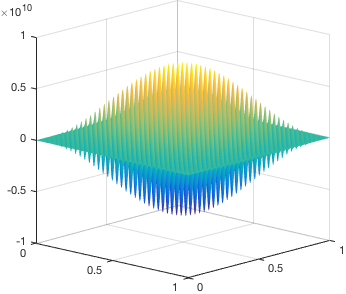
\includegraphics[width = 9cm]{explode_3D.png}
	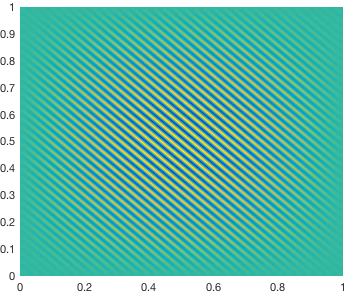
\includegraphics[width = 9cm]{explode_flat.png}
}
\caption{The high-frequency Fourier harmonics are amplified by explicit scheme when $\mu > 1/4$.}
\label{figure:explode}
\end{figure}
Let us have a deeper insight into the behaviour of explicit scheme. Suppose that $\mu_x + \mu_y > 1/2$. Recall that the amplification factor of $U_{j,k}^m =\lambda_{\alpha}^me^{i(\alpha_xx_j+\alpha_yy_k)}$ is
$$
\lambda_\alpha = 1 - 4\left(\mu_x\sin^2\frac{\alpha_xh_x}{2}+\mu_y\sin^2\frac{\alpha_yh_y}{2}\right)
$$
When $\alpha_x = N_x \pi/X$ and $\alpha_y = N_y \pi/Y$ the amplification factor reaches its maximum in absolute value. Therefore, the harmonics most prone to instability are those
with the highest spatial frequency, for which
$$
\sin^2\frac{\alpha_xh_x}{2} = \sin^2\frac{\alpha_yh_y}{2} = 1
$$
Note that the high-frequency wave \textbf{always} exists due to round-off error, so it's necessary to require $\mu_x + \mu_y < 1/2$ to ensure stability with any initial value.
 As is shown in figure \ref{figure:explode}, when $\mu_x > 1/4$ the high-frequency wave is amplified by the explicit scheme and grows at an exponential speed. 

We further explore the numerical schemes' potential with given space step size. We test each each numerical scheme with time step $k$ ranging from $1/4194304 = 1/2^{22}$ to $1/256 = 1/2^8$ and choose the best convergence result. As is shown in figure \ref{figure:plot}, the accuracy of the numerical schemes is roughly proportional to the space step $h$. Though explicit scheme imposes a restriction of $k \le h^2/4$ on the time step and is hence computationally
inefficient, it does have the highest accuracy as long as $k$ is small enough.
\begin{figure}[!htb]
\centerline{
	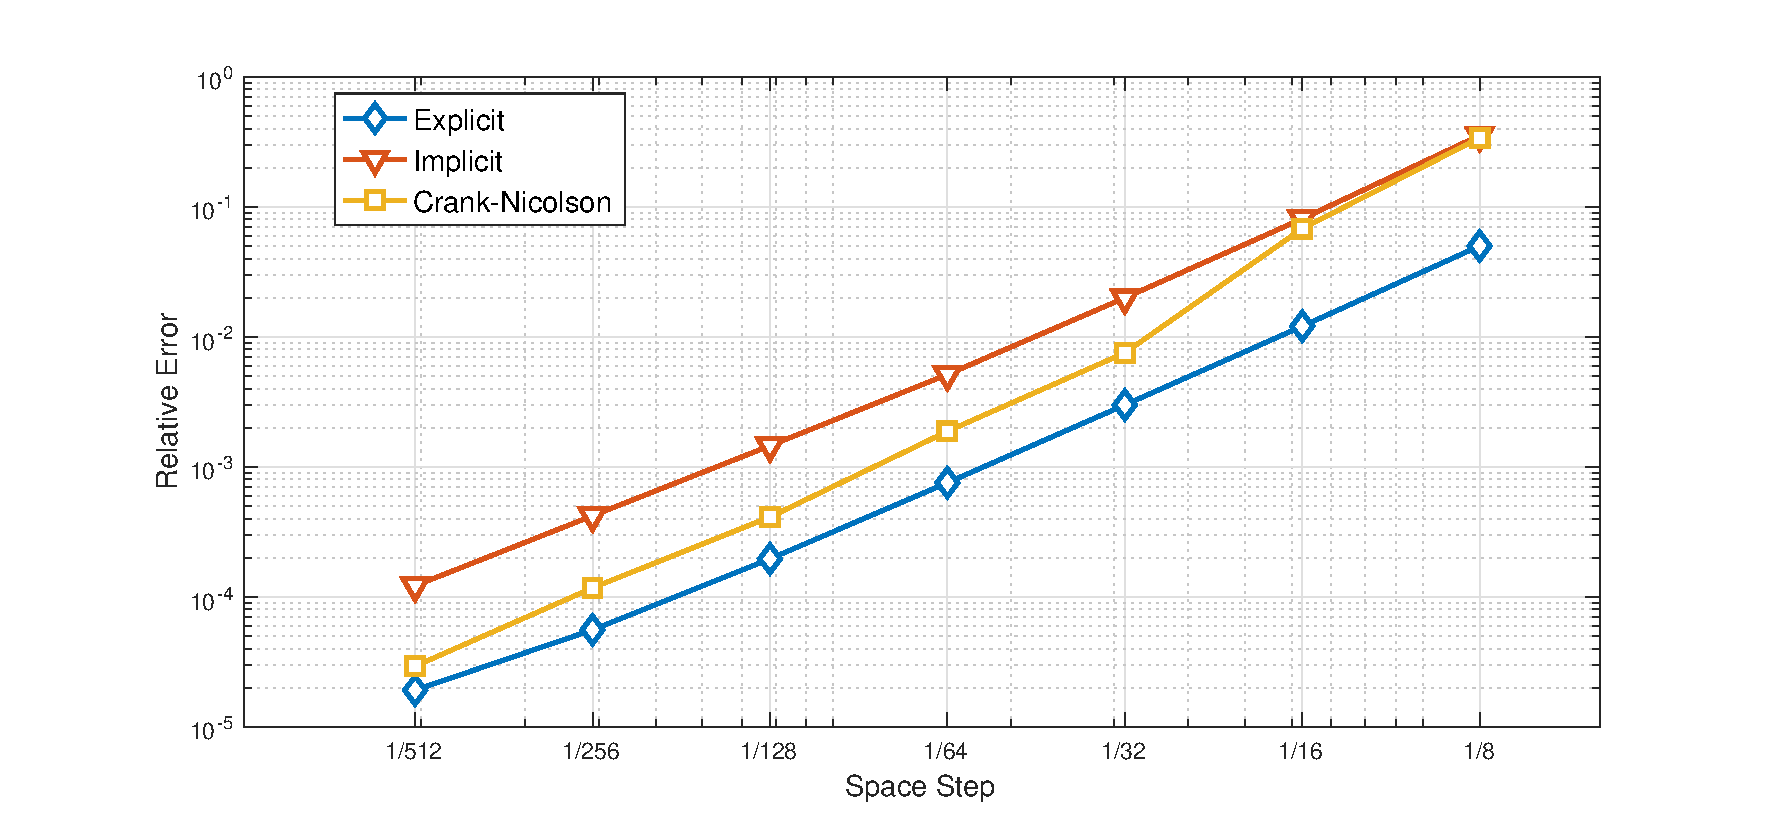
\includegraphics[width =20cm]{plot.eps}
}
\caption{The best convergence result at $t = 1$ of different numerical schemes with given space step size.}
\label{figure:plot}
\end{figure}

\subsection{Speed Test}
In this section, we compare the speed of four numerical methods for solving linear equations of the implicit scheme, namely, Multi Grid V method, Cholesky-Decomposition-based method, Gauss-Seidel method and conjugate gradient method. We focus on the CPU run time that each method costs to iterate from $t = 0$ to $t = 1$. The stopping criterion of each iteration is that the current residue reaches 1e-6 of the initial residue. 

As is shown in table \ref{table:CPU time}, the conjugate gradient method outperforms other three methods by a large margin. The run time of Multi Grid is roughly proportional to the linear equation's scale ($N^2$) while performing a Cholesky decompositon calls for $N^6/3$ flops, so the Multi Grid method outperforms Cholesky method when the space step $h$ gets smaller. 
\begin{table}[h]
\centerline{
\begin{tabular}{|c|c|c|cc|c|c|}
\hline
\multirow{2}*{Time Step $k$}& \multirow{2}*{Space Step $h$} & \multicolumn{5}{c|}{CPU time of different methods (sec)}\\
\cline{3-7}
 & & Multi Grid V& Cholesky &built-in function& Gauss-Seidel& Conjugate Gradient\\
\hline
\hline
\multirow{3}*{1/128} &   1/64  & 0.493 & 0.452 & {\color{blue}0.341} & 7.068 & {\color{red}0.326} \\
\cline{2-7}
&   1/128  & 1.581 & 2.791 & {\color{blue}1.449} & 159.715 & {\color{red}0.726} \\
\cline{2-7}
&   1/256  & {\color{blue}5.530} & 17.602 & 8.989 & 2632.407 & {\color{red}2.362} \\
\hline
\hline
\multirow{3}*{1/256} & 1/64  & 0.779 & 0.686 & {\color{blue}0.554} & 7.605 & {\color{red}0.420}  \\
\cline{2-7}
& 1/128  & 2.947 & 3.938 & {\color{blue}2.595} & 173.496 & {\color{red}0.954} \\
\cline{2-7}
& 1/256  & {\color{blue}10.571} & 29.444 & 15.943 & 2779.432 & {\color{red}3.255} \\
\hline
\hline
\multirow{3}*{1/512} & 1/64  & 1.046 & 0.949 & {\color{blue}0.860} & 8.036 & {\color{red}0.534} \\
\cline{2-7}
& 1/128  & {\color{blue}4.167} & 5.871 & 4.563 & 180.672 & {\color{red}1.090} \\
\cline{2-7}
& 1/256  & {\color{blue}15.717} & 43.194 & 30.924& 2856.276 & {\color{red}4.634} \\
\hline
\end{tabular}}
\caption{CPU run time of different numerical methods, the best result. {\color{red}Red color} indicates the best performance and {\color{blue}blue color} indicates the second best performance.}
\label{table:CPU time}
\end{table}

\begin{figure}[!htb]
\centerline{
	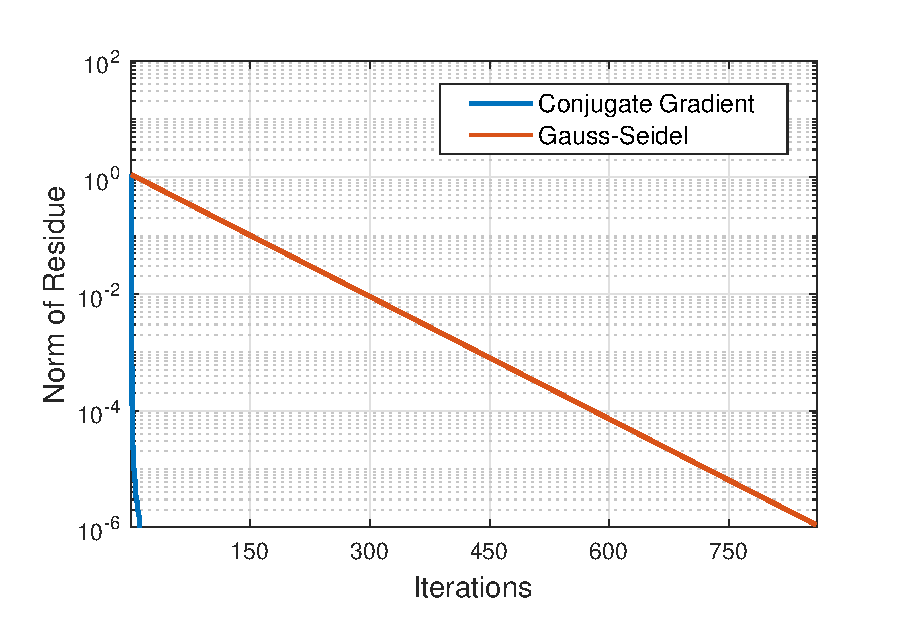
\includegraphics[width = 10cm]{CG_GS.eps}
	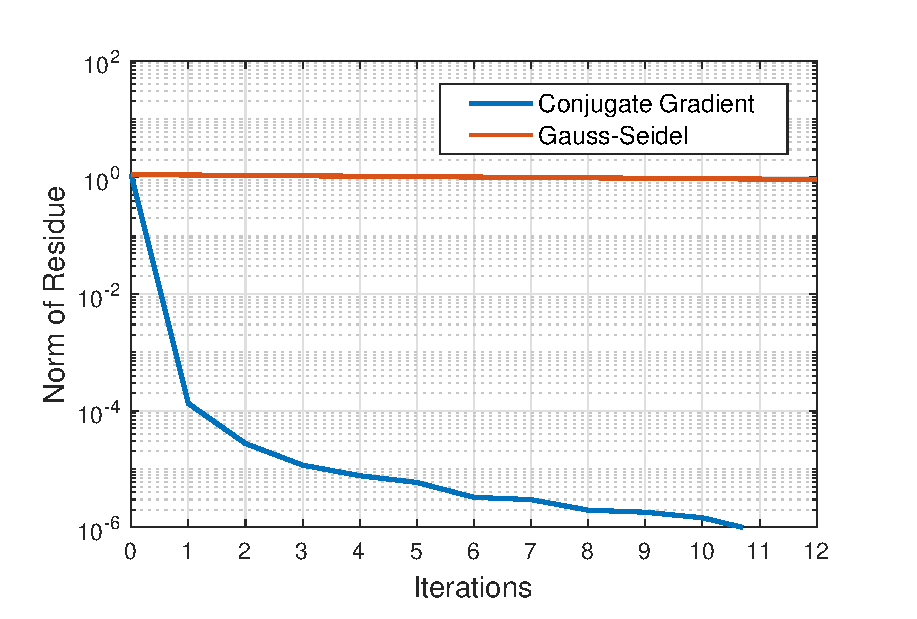
\includegraphics[width = 10cm]{CG_GS_zoom.eps}
}
\caption{Norm of residue V.S. iteration number in sub-problem}
\label{fig:CG_GS}
\end{figure}
Note that the analytical solution is $u = e^{-2\pi^2t}\sin(\pi x)\sin(\pi y)$, so actually we have 
$$
\vec{U}^{m+1}\approx e^{-2\pi^2k}\vec{U}^m
$$
When we choose $\vec{U}^m$ as the inital value in the linear equation $Ax = b = \vec{U}^m$, the negative gradient of $x^{\rm T}Ax - 2bx$ at $\vec{U}^m$ is given by 
$$
-2(A\vec{U}^m - \vec{U}^m) \approx -2(e^{2\pi^2k}A\vec{U}^{m+1} - \vec{U}^m) = -2(e^{2\pi^2k}-1)\vec{U}^m \approx 2\frac{e^{2\pi^2k}-1}{1-e^{-2\pi^2k}}\left(\vec{U}^{m+1} - \vec{U}^m\right)
$$
which points directly from $\vec{U}^{m}$ to $\vec{U}^{m+1}$, so we can get an accurate solution with merely one iteration in conjugate gradient method. As is shown in figure \ref{fig:CG_GS}, the norm of residue decreases from 1.1149 to 1.324e-4 at the first iteration, which matches our speculation. This may help to explain why CG method performs so well in this problem. As for Gauss-Seidel method, the convergence speed depends on the spectral radius of $(D-L)^{-1}U$, which is approximate $0.98396$ when $h = 1/128$ and $k = 1/512$. It could be caused by the special structure of $\bar{L}_{h_x,h_y}$. 
\end{document}